% ----------------------------------------------------------
% Metodologia
% ----------------------------------------------------------
\chapter{Metodologia} \label{sec:metodologia}

Este capítulo descreve os materiais e métodos utilizados no desenvolvimento do aplicativo. 

\section{Metodologia de desenvolvimento} \label{sec:metodologia de desenvolvimento} 

No desenvolvimento do presente trabalho, foram utilizados os princípios das metodologias ágeis que têm como objetivo acelerar, adaptar e visar o melhor processo para o desenvolvimento do software, entregando o produto final  ao cliente com o que realmente deseja e com qualidade. Dentre dos modelos de processos ágeis, foi abordado o modelo de desenvolvimento de software enxuto.

O Desenvolvimento de Software Enxuto ou \textit{Lean Software Development} (LSD),
de acordo com \citeauthor{poppendiek2003}, é a aplicação dos princípios da \textit{Toyota Product Development System}  para o desenvolvimento de software que, quando aplicado de forma correta, possibilita alta qualidade, rapidez e baixo custo. Para atingir esse objetivo, o modelo de desenvolvimento Lean possui alguns princípios, Figura \ref{fig:principios-lean}. 


\begin{figure}[H]
	\caption{\label{fig:principios-lean}Princípios do modelo Lean}
	\centering
	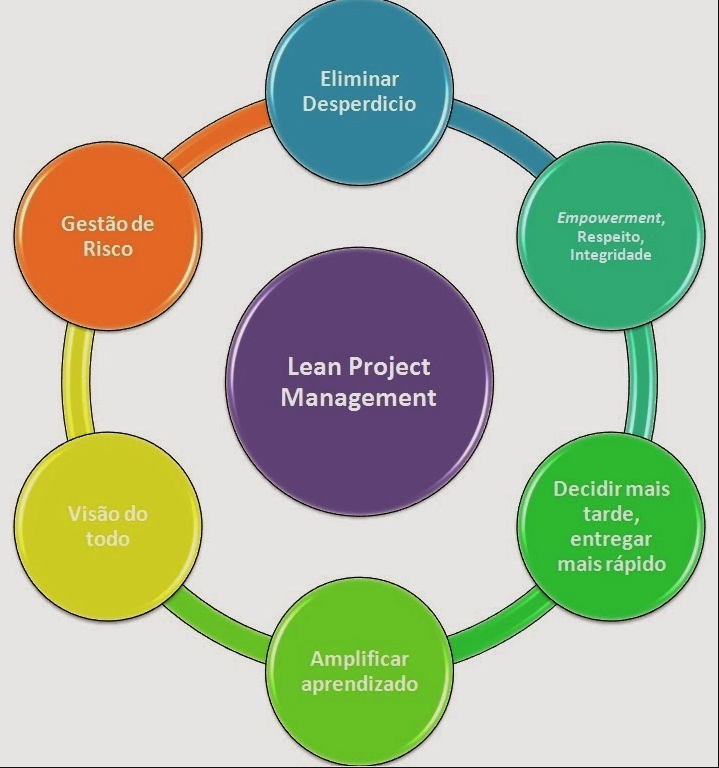
\includegraphics[scale=0.3]{imagens/figura7.png}
	\legend{Fonte: \citeauthor{rosamilha2014}}
\end{figure}

\section{Ferramentas e tecnologias utilizadas} \label{sec:ferramentas} 
Nesta seção, iremos apresentar alguns dos materiais que foram necessários para o desenvolvimento deste trabalho.


\subsection{Ionic Framework}

Ionic é uma combinação de tecnologias e utilitários projetados para tornar a construção de aplicativos móveis híbridos de forma rápida, fácil e bonita. Ele foi criado pela DriftyCo em 2012 e consiste em uma compilação de várias ferramentas que possibilitam o desenvolvimento de aplicações utilizando tecnologias e linguagens de programação web como HTML, CSS e Javascript.

Através do \citeauthor{ionic2017} Framework é possível desenvolver aplicações móveis híbridas com interface e a utilização de recursos das três plataformas mais utilizadas: Android, IOS e Windows Phone. Esse Framework também possibilita o desenvolvedor criar aplicações progressivas, que são websites móveis que possuem performance próxima da performance de um aplicativo nativo.

\subsection{Angular JS}
\citeauthor{angularjs2017} é um framework SPA (\textit{Single Page Applications}) em Javascript, de código aberto e mantido pelo Google,
que permite escrever aplicativos Web. Ele permite que você use HTML como sua linguagem de modelo e permite expandir a sintaxe do HTML para expressar os componentes da sua aplicação de forma clara e sucinta. A ligação de dados e a injeção de dependência da AngularJS eliminam muito do código que de outra forma você teria que escrever.

O Angular JS disponibiliza recursos completos para facilitar a criação de um aplicativo CRUD: 
\begin{lista}
	\item Vinculação de dados;
	\item Diretrizes básicas de modelos;
	\item Validação de formulários; 
	\item Roteamento;
	\item Componentes reutilizáveis;
	\item Injeção de dependência.
\end{lista}

\subsection{Ruby}

\citeauthor{ruby2017} é uma linguagem orientada a objetos, com tipagem forte e dinâmica criada por Yukihiro "Matz" Matsumoto, que misturou partes de suas linguagens favoritas (Perl, Smalltalk, Eiffel, Ada e Lisp) para formar uma nova linguagem com objetivo de ser uma linguagem simples de ler e ser entendida, para facilitar o desenvolvimento e manutenção de sistemas escritos com ela. Possui vários repositórios de bibliotecas disponíveis em sites como \textit{Ruby Forge} e \textit{Ruby Application Archive} (RAA). Existe, ainda, uma ferramenta bastante útil para instalação de bibliotecas, chamada \textit{Ruby Gems}. O software mais conhecido desenvolvido em Ruby é o \citeauthor{rubyonrails}.

\subsection{Facebook SDK}

O \citeauthor{facebooksdk} (Software Development Kit) está inserido em uma plataforma: a \textit{Facebook Platform}. Essa plataforma permite que qualquer um construa aplicativos sociais no Facebook e na Web, disponibilizando uma coleção abrangente de APIs e SDKs.

A principal API (\textit{Application Program Interface}) do Facebook Platform é API \textit{Graph}, que permite aos desenvolvedores criarem seus próprios aplicativos. Através desta API as aplicações podem acessar e reunir informações sobre o usuário (desde que o usuário tenha permitido o acesso as suas informações). 

A classe principal do Facebook SDK encapsula métodos que permitem autorizar o usuário, criar diálogos do Facebook, fazer solicitações de API, desconectar o usuário e ter ou definir informações de acesso e sessão, além do status. Quando os usuários acessam a aplicação,  poderão conceder permissões para que o aplicativo possa recuperar informações ou executar alguma ação no Facebook, no nome do usuário.

